% Provenance (never printed): see sources/outline_sources.md (Year 3:
% speciation and saturation indices; carbonate equilibria applied to rocks;
% weathering kinetics; hydrothermal fluids). Brief: sources/book5/BRIEFS.md,
% ch. 15. Curves from figdata/bachelor-3/carbonate_system.py,
% activity_diagram.py, weathering_rates.py. Exercise and problem values in the
% Book 5 scratch calculator calc/ch15.py. The spring below the Varden
% limestone, its analysis and the granite stream are invented.
\chapter{Interaksi Air--Batuan}\label{ch:b3:water-rock-interaction}

Sebuah mata air di kaki tebing batu gamping meninggalkan kerak putih pada setiap
ranting dan batu yang disentuhnya; sebuah sungai yang mengalir dari granit membawa
silika, natrium, dan sedikit kalium, dan sama sekali tidak meninggalkan kerak. Perbedaannya
terletak pada kimia air, dan kimia itu adalah catatan tentang batuan
yang dilewati air: berapa banyak karbon dioksida yang dibawanya, berapa lama ia
tinggal, mineral mana yang dilarutkannya dan mana yang dibentuknya. Bab ini
membaca catatan itu dengan perangkat kimia larutan, mulai dari analisis sebuah
air hingga laju pelarutan mineral dan jejak isotop dari fluida panas di kerak.

\begin{recall}
Aktivitas, koefisien aktivitas, kekuatan ion, spesiasi, hasil kali
kelarutan, alkalinitas, keadaan kejenuhan $\Omega$, hukum Henry, hukum laju,
hukum Arrhenius, keadaan transisi, dan nilai $\delta$ dibahas dalam
volume universitas buku kimia. Pelapukan kimia, hidrolisis
silikat, mineral lempung, dan kaolinit ada dalam volume Tahun 1, pada
bab tentang pelapukan dan lempung; lisoklin dan kedalaman
kompensasi karbonat pada bab tentang sedimen karbonat, silisiklastik, dan evaporit. Fluida
hidrotermal ada dalam volume Tahun 2, pada bab tentang endapan bijih, dan
termostat pelapukan silikat pada bab tentang iklim sepanjang waktu geologi; sirkulasi
hidrotermal ada dalam buku-buku sekolah.
\end{recall}

\section{Analisis air alami}\label{sec:b3:water-rock-interaction:analysis}

Analisis air mencantumkan ion-ion mayor dalam miligram per liter: kalsium,
magnesium, natrium, dan kalium; bikarbonat, klorida, sulfat, dan nitrat;
silika terlarut sebagai \ce{SiO2}; serta pH dan suhu yang diukur di
sumber air, karena keduanya berubah begitu sampel meninggalkan sumbernya. Membagi dengan
massa molar menghasilkan milimol per liter, dan mengalikannya dengan muatan
menghasilkan miliekuivalen. Air encer bersifat netral secara listrik, sehingga
jumlah kation harus sama dengan jumlah anion.

\begin{method}[Memeriksa analisis air]\label{met:b3:water-rock-interaction:analysis}
\begin{enumerate}
\item ubah setiap konsentrasi menjadi \unit{mmol/L} dan \unit{meq/L};
\item jumlahkan kation dan anion dalam \unit{meq/L};
\item hitung galat keseimbangan muatan $100\,(\sum\text{kation} -
  \sum\text{anion})/(\sum\text{kation} + \sum\text{anion})$, dalam persen;
\item terima analisis jika galatnya berada dalam 1 atau \qty{2}{\percent} untuk
  air dengan 250 sampai \qty{1000}{mg/L}, sedikit lebih besar untuk air yang
  lebih encer; jika tidak, cari ion yang hilang atau galat analitik.
\end{enumerate}
\end{method}
% ledger: hem85:charge-balance

Aktivitas sebuah ion adalah molalitasnya dikali koefisien aktivitasnya
$\gamma$. Dalam air alami $\gamma$ dihitung dari kekuatan ion $I =
\tfrac12\sum m_i z_i^2$ dengan persamaan Debye--Hückel yang diperluas
\[
-\log\gamma_i = \frac{A z_i^2\sqrt I}{1 + B a_i\sqrt I},
\]
dengan $A = 0.5085$ dan $B = 0.3281$ untuk air pada \qty{25}{\celsius}, dan
ukuran ion $a_i$ dalam ångström: 9 untuk \ce{H+}, 8 untuk \ce{Mg^2+}, 6 untuk
\ce{Ca^2+}, 5 untuk \ce{CO3^2-}, 4 untuk \ce{Na+}, \ce{HCO3-} dan \ce{SO4^2-},
3 untuk \ce{K+}, \ce{Cl-}, \ce{OH-} dan \ce{NO3-}. Persamaan ini berlaku hingga
sekitar \qty{0.1}{mol/L} garam univalen, yang mencakup sungai dan sebagian besar
air tanah, tetapi tidak air laut atau larutan garam pekat. Suhu hanya mengubah
$A$ dari 0.4883 pada \qty{0}{\celsius} menjadi 0.5425 pada \qty{60}{\celsius},
sehingga nilai pada \qty{25}{\celsius} juga cukup untuk air dingin.
% ledger: hem85:debye-huckel

Karbon anorganik dalam air terbagi di antara karbon dioksida terlarut
(ditulis \ce{CO2} untuk jumlah \ce{CO2} dan \ce{H2CO3}), bikarbonat, dan
karbonat, yang dihubungkan oleh
\[
K_1 = \frac{a_{\ce{HCO3-}}\,a_{\ce{H+}}}{a_{\ce{CO2}}}, \qquad
K_2 = \frac{a_{\ce{CO3^2-}}\,a_{\ce{H+}}}{a_{\ce{HCO3-}}}, \qquad
K_H = \frac{a_{\ce{CO2}}}{P_{\ce{CO2}}},
\]
dengan $\log K_1 = -6.35$, $\log K_2 = -10.33$, dan $\log K_H = -1.47$ pada
\qty{25}{\celsius}, serta $-6.46$, $-10.49$, dan $-1.27$ pada \qty{10}{\celsius}
($P$ dalam atmosfer). Di antara pH 6.4 dan 10.3 bikarbonat mendominasi, dan
di sebagian besar air alami alkalinitas hampir seluruhnya bikarbonat. Dengan pH
dan bikarbonat yang terukur, kita memperoleh dua spesies lainnya, serta tekanan
parsial karbon dioksida yang berada dalam kesetimbangan dengan air itu.
% ledger: phreeqc:carbonate

\section{Kejenuhan}\label{sec:b3:water-rock-interaction:saturation}

\begin{definition}[Indeks kejenuhan]\label{def:b3:water-rock-interaction:si}
Yang disebut \emph{indeks kejenuhan}\index{indeks kejenuhan}
dalam sebuah air adalah $\mathrm{SI} = \log(\mathrm{IAP}/K)$, dengan IAP
adalah hasil kali aktivitas ion dalam air yang ditulis seperti hasil kali
kelarutan mineral $K$: $\mathrm{SI} = \log\Omega$.
\end{definition}

Air dengan $\mathrm{SI} < 0$ dapat melarutkan mineral, air dengan
$\mathrm{SI} > 0$ dapat mengendapkannya, dan $\mathrm{SI} = 0$ berarti kesetimbangan.
Karena energi bebas reaksi pelarutan adalah $\Delta_r G = RT\ln\Omega
= 2.303\,RT\,\mathrm{SI}$, \omterm{def:b3:water-rock-interaction:si}{indeks kejenuhan} juga merupakan ukuran gaya pendorong,
dalam satuan $2.303\,RT$, sekitar \qty{5.7}{kJ/mol} pada
\qty{25}{\celsius}. Untuk kalsit $\mathrm{IAP} = a_{\ce{Ca^2+}}
a_{\ce{CO3^2-}}$ dan $\log K = -8.45$ pada \qty{25}{\celsius}, $-8.35$ pada
\qty{10}{\celsius}: kalsit lebih mudah larut di air dingin. Untuk gipsum, $\mathrm{SI} = \log(a_{\ce{Ca^2+}}a_{\ce{SO4^2-}}) + 4.55$;
untuk kuarsa, yang pelarutannya menghasilkan \ce{H4SiO4} netral, $\mathrm{SI} = \log
a_{\ce{H4SiO4}} + 3.98$, dan untuk silika amorf konstantanya 2.71
alih-alih 3.98. Indeks terukur memiliki ketidakpastian sedikitnya $\pm0.1$,
dan air yang berada dalam $\pm0.3$ dari nol dianggap mendekati kesetimbangan.
% ledger: phreeqc:carbonate, phreeqc:silicates, hem85:si

\section{Kesetimbangan karbonat dalam batuan}\label{sec:b3:water-rock-interaction:carbonate}

Kalsit larut dalam air yang diisi karbon dioksida menurut
\[
\ce{CaCO3 + CO2 + H2O <=> Ca^2+ + 2 HCO3-},
\qquad K = \frac{a_{\ce{Ca^2+}}\,a_{\ce{HCO3-}}^2}{P_{\ce{CO2}}}
= \frac{K_{\mathrm{cal}}K_1K_H}{K_2},
\]
dengan $\log K = -5.94$ pada \qty{25}{\celsius} dan $-5.59$ pada \qty{10}{\celsius}.
Seberapa banyak yang larut bergantung pada asal karbon dioksidanya.

\begin{definition}[Sistem karbonat terbuka dan tertutup]\label{def:b3:water-rock-interaction:open-closed}
Air melarutkan kalsit dalam \emph{sistem karbonat terbuka}\index{sistem karbonat terbuka}
ketika air tetap bersentuhan dengan gas dengan tekanan parsial
$P_{\ce{CO2}}$ yang tetap, yang menggantikan karbon dioksida yang terpakai. Ia melakukannya dalam
\emph{sistem karbonat tertutup}\index{sistem karbonat tertutup} ketika air
lebih dahulu diisi karbon dioksida lalu diisolasi dari gas, sehingga
karbon dioksida yang dikandungnya merupakan seluruh yang dapat dipakainya.
\end{definition}

\begin{theorem}[Kelarutan kalsit, terbuka dan tertutup]\label{thm:b3:water-rock-interaction:calcite}
Untuk air bertipe kalsium bikarbonat, dengan $m$ molalitas kalsium,
\[
\text{terbuka:}\quad m = \left(\frac{K\,P_{\ce{CO2}}}{4\gamma_{\ce{Ca^2+}}
\gamma_{\ce{HCO3-}}^2}\right)^{1/3};
\qquad
\text{tertutup:}\quad 4\gamma_{\ce{Ca^2+}}\gamma_{\ce{HCO3-}}^2\,m^3 =
\frac{K_{\mathrm{cal}}K_1}{K_2}\,(C_0 - m),
\]
dengan $C_0 = K_H P_{\ce{CO2}}$ adalah karbon dioksida yang terserap sebelum
sistem ditutup.
\end{theorem}

\begin{proof}
Antara pH 6.5 dan 8.5 karbonat, \ce{H+} dan \ce{OH-} dapat diabaikan dibanding
bikarbonat, sehingga keseimbangan muatannya $2m = m_{\ce{HCO3-}}$. Terbuka: $K = \gamma
_{\ce{Ca^2+}}m\,\gamma_{\ce{HCO3-}}^2(2m)^2/P_{\ce{CO2}}$, yang memberikan
akar pangkat tiga. Tertutup: setiap kalsium yang larut memakai satu \ce{CO2}, sehingga $m_{\ce{CO2}}
= C_0 - m$ dan $a_{\ce{Ca^2+}}a_{\ce{HCO3-}}^2/a_{\ce{CO2}} = K/K_H =
K_{\mathrm{cal}}K_1/K_2$ memberikan persamaan pangkat tiga.
\end{proof}

Pada sistem terbuka kalsium tumbuh sebagai akar pangkat tiga dari $P_{\ce{CO2}}$; pada
sistem tertutup kalsium dibatasi oleh $C_0$, dan karbon dioksida yang tersisa di
akhir, sehingga $P_{\ce{CO2}}$ akhirnya jauh lebih rendah daripada di awal. Udara tanah
mengandung 10 sampai 100 kali karbon dioksida atmosfer, dihasilkan oleh akar
dan oleh dekomposisi bahan tanaman, dan air tanah umumnya menunjukkan
$P_{\ce{CO2}}$ antara $10^{-2.5}$ dan $10^{-1}$ atmosfer. Air yang bersentuhan
dengan kalsit dan udara hanya memuat sekitar \qty{20}{mg/L} kalsium; hujan yang
mencapai batu gamping melalui tanah, masih terbuka terhadap gas tanah, dapat
mengambil empat atau lima kali lebih banyak. Karst terbentuk oleh karbon dioksida tanah ini.
% ledger: hem85:pco2, phreeqc:carbonate

Jalan kembalinya adalah pelepasan gas. Mata air yang muncul dari batu gamping
membawa $P_{\ce{CO2}}$ dari tanah dan batuan, sepuluh sampai seratus kali lebih besar daripada
udara. Di tempat terbuka ia kehilangan karbon dioksida, bikarbonat berubah menjadi
karbonat, pH naik, dan \omterm{def:b3:water-rock-interaction:si}{indeks kejenuhan} naik lebih dari satu satuan,
seperti ditunjukkan panel (b) pada gambar di bawah untuk mata air dalam
soal akhir pekan bab ini.
Kalsit mengendap di dasar aliran dan pada lumut serta ranting: tufa dari
mata air dingin, travertin dari mata air panas. Mata air yang melewati batuan
dengan cepat, dalam hitungan hari atau minggu, melalui saluran, umumnya mencapai permukaan
dalam keadaan tak jenuh; yang merembes perlahan melaluinya selama berbulan-bulan muncul mendekati
kejenuhan.
% ledger: hem85:pco2, usgsyvo:travertine

\begin{omfigure}
\begin{tikzpicture}
\begin{groupplot}[group style={group size=2 by 1, horizontal sep=1.6cm},
  omrecord, width=0.47\linewidth, height=0.42\linewidth, title style={font=\small},
  tick label style={font=\scriptsize}, label style={font=\small},
  legend style={font=\scriptsize, legend cell align=left}]
\nextgroupplot[title={(a) kelarutan kalsit},
  xlabel={$\log P_{\ce{CO2}}$ (atm)}, ylabel={kalsium terlarut (\unit{mmol/L})},
  xmin=-3.5, xmax=-1, ymin=0, ymax=5.5, clip=false,
  xtick={-3.5,-3,-2.5,-2,-1.5,-1}, xticklabels={$-3.5$,$-3$,$-2.5$,$-2$,$-1.5$,$-1$},
  legend style={at={(0.14,0.97)}, anchor=north west}]
\addplot[draw=none, fill=black!6, forget plot] coordinates {(-2.5,0) (-2.5,5.5) (-1,5.5) (-1,0)} -- cycle;
% computed in figdata/bachelor-3/carbonate_system.py
\addplot[omDef, thick] table[x=logp, y=ca_open10] {figdata/out/bachelor-3-carbonate_system-solubility.dat};
\addlegendentry{terbuka, \qty{10}{\celsius}}
\addplot[red!70!black, thick] table[x=logp, y=ca_open25] {figdata/out/bachelor-3-carbonate_system-solubility.dat};
\addlegendentry{terbuka, \qty{25}{\celsius}}
\addplot[omDef, thick, densely dashed] table[x=logp, y=ca_closed10] {figdata/out/bachelor-3-carbonate_system-solubility.dat};
\addlegendentry{tertutup, \qty{10}{\celsius}}
\addplot[red!70!black, thick, densely dashed] table[x=logp, y=ca_closed25] {figdata/out/bachelor-3-carbonate_system-solubility.dat};
\addlegendentry{tertutup, \qty{25}{\celsius}}
\draw[black, densely dotted] (axis cs:-3.37,0) -- (axis cs:-3.37,5.5);
\node[font=\scriptsize, anchor=south] at (axis cs:-3.37,5.5) {udara};
\node[font=\scriptsize, anchor=north] at (axis cs:-1.4,5.45) {air tanah};
\nextgroupplot[title={(b) mata air yang melepaskan gas},
  xlabel={$\log P_{\ce{CO2}}$ (atm)}, ylabel={SI kalsit},
  xmin=-3.5, xmax=-1.5, ymin=-0.2, ymax=1.9, x dir=reverse, clip=false,
  xtick={-3.5,-3,-2.5,-2,-1.5}, xticklabels={$-3.5$,$-3$,$-2.5$,$-2$,$-1.5$}]
% computed in figdata/bachelor-3/carbonate_system.py
\addplot[omDef, thick] table[x=logp, y=si] {figdata/out/bachelor-3-carbonate_system-degassing.dat};
\addplot[black, densely dotted, domain=-3.5:-1.5, samples=2] {0};
\addplot[red!70!black, only marks, mark=*, mark size=1.6pt] table[x=logp, y=si] {figdata/out/bachelor-3-carbonate_system-ends.dat};
\node[font=\scriptsize, anchor=north west] at (axis cs:-1.84,-0.01) {keluaran};
\node[font=\scriptsize, anchor=north west] at (axis cs:-3.3,1.55) {udara};
\end{groupplot}
\end{tikzpicture}

\par\smallskip{\small (a) Kalsium yang terlarut oleh air dalam kesetimbangan dengan
kalsit, terhadap tekanan parsial karbon dioksida (untuk sistem tertutup,
tekanan tempat air diisi): sistem terbuka garis padat, sistem tertutup
putus-putus; air dingin melarutkan lebih banyak; pita abu-abu adalah rentang
air tanah. (b) Mata air di bawah batu gamping Varden, pada \qty{10}{\celsius},
melepaskan karbon dioksida saat turun bukit (dibaca dari kiri ke kanan, pada sumbu terbalik)
sebelum kalsit terbentuk: kalsium dan alkalinitasnya tetap, pH-nya naik
dari 7.2 menjadi 8.8, dan \omterm{def:b3:water-rock-interaction:si}{indeks kejenuhannya} dari 0.04 menjadi 1.6. Konstanta
kesetimbangan dari basis data publik, serta koefisien aktivitas Debye--Hückel
diperluas.}\label{fig:b3:water-rock-interaction:calcite}
\end{omfigure}
% ledger: phreeqc:carbonate, hem85:debye-huckel, hem85:pco2, data:co2-mlo

Kimia yang sama, bila dijalankan pada skala samudra, dibahas dalam
volume universitas buku kimia; kedalaman tempat air laut menjadi tidak jenuh
terhadap kalsit, yaitu lisoklin, dan kedalaman di bawahnya kalsit tidak
lagi terakumulasi, dibahas dalam volume Tahun 1.

\begin{inthefield}[Mata air yang membangun teras sendiri]
\begin{minipage}[t]{0.52\linewidth}\vspace{0pt}
Di Palette Spring, salah satu Mammoth Hot Springs di dataran tinggi
Yellowstone, air panas naik melalui batu gamping terkubur dan membawanya pergi
dalam keadaan terlarut. Di permukaan, air
menyebar di atas endapannya sendiri dan kehilangan karbon dioksida, lalu kalsium karbonat
mengendap sebagai travertin, pertama di tepi setiap kolam, tempat air paling
tipis. Ahli geologi yang menyurvei mata air ini mengukur pengendapan sekitar
tiga milimeter per hari, lima belas kali laju tufa mata air dingin.
Garis-garis jingga dan
cokelat adalah hamparan mikroba pencinta panas yang hidup di limpasan hangat.
\end{minipage}\hfill
\begin{minipage}[t]{0.44\linewidth}\vspace{0pt}
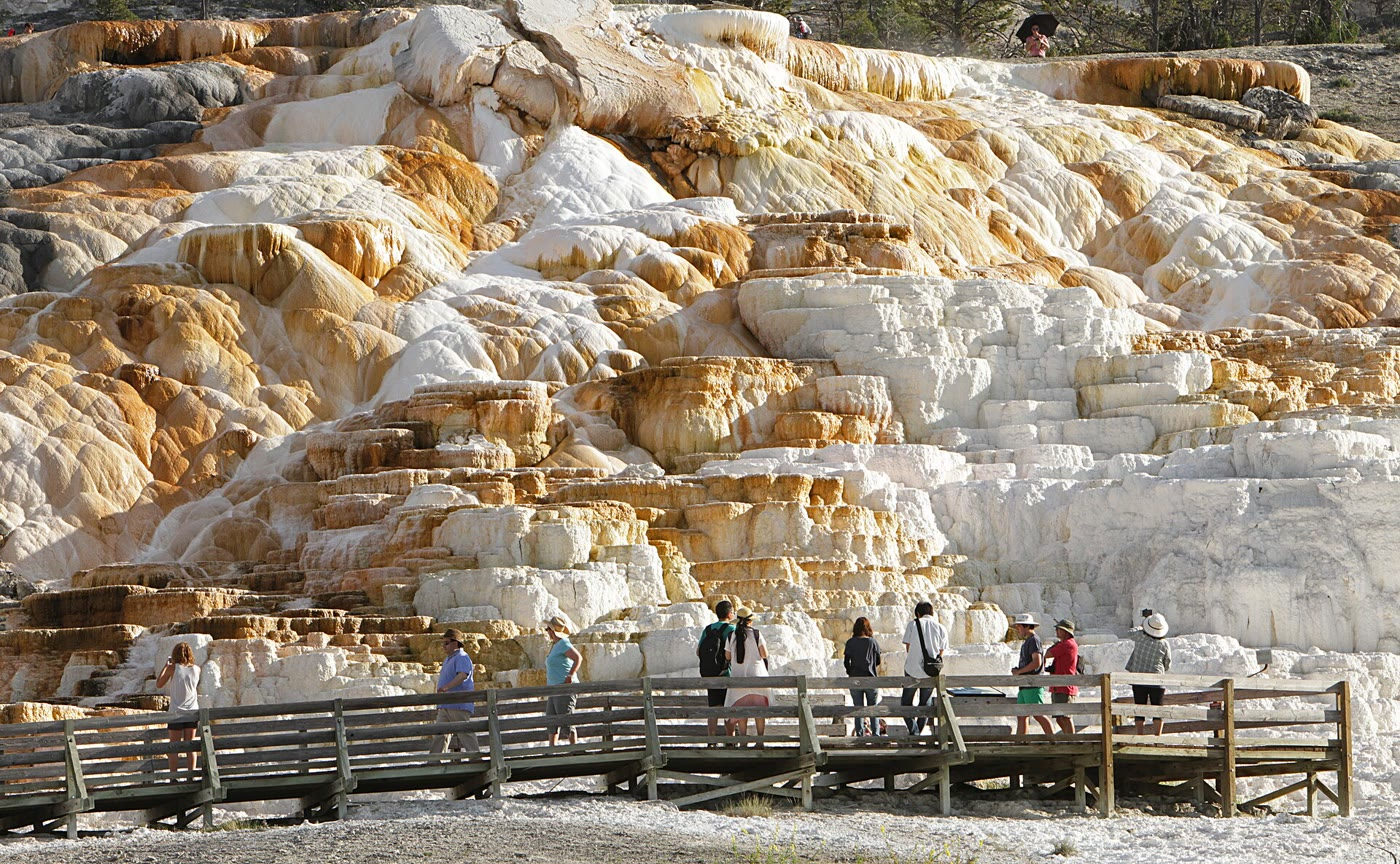
\includegraphics[width=\linewidth]{images/book5/b3-palette-spring-travertine.jpg}

{\scriptsize Teras travertin Palette Spring, Mammoth Hot Springs, dengan
jalur kayu dan pengunjung sebagai pembanding skala. Foto NPS oleh Jim Peaco, domain publik.}
\end{minipage}
\end{inthefield}
% ledger: photo:b3-palette-spring, usgsyvo:travertine, nps:travertine-terraces

\section{Kinetika pelapukan silikat}\label{sec:b3:water-rock-interaction:kinetics}

Silikat larut jauh lebih lambat daripada kalsit, dan air jarang mencapai
kesetimbangan dengan silikat: pelarutannya harus dinyatakan dengan suatu laju.

\begin{definition}[Hukum laju pelarutan mineral]\label{def:b3:water-rock-interaction:rate-law}
Yang disebut \emph{hukum laju pelarutan mineral}\index{hukum laju pelarutan mineral}
memberikan laju pelarutan per satuan luas permukaan mineral, dalam
\unit{mol.m^{-2}.s^{-1}}, sebagai jumlah mekanisme asam, netral, dan basa,
\[
r = \sum_j k_j\,e^{-\frac{E_j}{R}\left(\frac1T - \frac1{298.15}\right)}\,
a_{\ce{H+}}^{n_j}\,\bigl(1 - \Omega^{p_j}\bigr)^{q_j},
\]
dengan konstanta laju $k_j$ pada \qty{25}{\celsius}, energi aktivasi $E_j$,
orde reaksi $n_j$ (negatif untuk mekanisme basa), dan dua eksponen
$p_j$, $q_j$, yang umumnya diambil bernilai 1.
\end{definition}
% ledger: pk04:rate-law

\begin{proposition}[Jauh dari dan dekat kesetimbangan]\label{prop:b3:water-rock-interaction:affinity}
Dengan $p = q = 1$, laju tidak bergantung pada kejenuhan air
bila $\Omega \ll 1$, dan dekat kesetimbangan laju itu sebanding dengan
\omterm{def:b3:water-rock-interaction:si}{indeks kejenuhan}: $r \approx -2.303\,r_\infty\,\mathrm{SI}$, dengan
$r_\infty$ adalah laju jauh dari kesetimbangan.
\end{proposition}

\begin{proof}
Faktornya adalah $1 - \Omega = 1 - 10^{\mathrm{SI}}$. Untuk $\mathrm{SI} \ll 0$ nilainya
mendekati 1; untuk $\mathrm{SI}$ dekat 0, $10^{\mathrm{SI}} \approx 1 +
2.303\,\mathrm{SI}$.
\end{proof}

Konstanta laju berasal dari eksperimen laboratorium pada bubuk mineral segar,
dalam reaktor alir yang dijaga jauh dari kesetimbangan. Gambar di bawah menggambarkan
hukum laju untuk empat mineral pada \qty{25}{\celsius}. Setiap kurva berbentuk V atau
U: proton mempercepat pelarutan dalam air asam, hidroksida dalam air basa, dan di
antara mekanisme netral menetapkan batas bawah. Olivin larut sekitar tiga
orde magnitudo lebih cepat daripada albit pada pH 5, itulah sebabnya ia menjadi
silikat umum pertama yang hilang dari tanah. Energi aktivasi albit dan
forsterit, 65 sampai \qty{79}{kJ/mol}, membuat laju keduanya empat sampai lima
kali lebih cepat pada \qty{25}{\celsius} dibanding pada \qty{10}{\celsius}.
% ledger: pk04:rates

Laju di lapangan lebih rendah, dengan selisih beberapa orde magnitudo. Dalam eksperimen kolom pada
granit yang baru dihancurkan, laju plagioklas turun secara stabil selama enam tahun
hingga \qty{7.0e-14}{mol.m^{-2}.s^{-1}}; granit yang sama, yang secara alami telah lapuk
dan sebagian berubah menjadi kaolinit, larut pada \qty{2.1e-15}{mol.m^{-2}.s^{-1}}
pada kondisi yang sama, dan keduanya masih jauh lebih cepat daripada laju
yang terukur di profil pelapukan itu sendiri. Dari banyak mineral dan umur, laju
menurun seiring waktu $t$ mineral itu telah mengalami pelapukan sebagai $R =
\num{3.1e-13}\,t^{-0.61}$ (mol\,m$^{-2}$\,s$^{-1}$, $t$ dalam tahun). Sebagian
penurunan terjadi pada mineralnya, yang permukaan paling reaktifnya larut lebih dulu;
sisanya terjadi pada lingkungannya: air yang lambat, banyak mineral untuk sedikit fluida, dan
air pori yang dekat dengan kesetimbangan, tempat proposisi di atas membuat laju
kecil.
% ledger: whitebrantley03:rates

\begin{omfigure}
\begin{tikzpicture}
\begin{axis}[omrecord, width=0.74\linewidth, height=0.46\linewidth,
  xlabel={pH}, ylabel={$\log r$ (\unit{mol.m^{-2}.s^{-1}})},
  xmin=0, xmax=14, ymin=-14.5, ymax=-6, clip=false,
  xtick={0,2,4,6,8,10,12,14}, ytick={-14,-12,-10,-8,-6},
  yticklabels={$-14$,$-12$,$-10$,$-8$,$-6$},
  tick label style={font=\scriptsize}, label style={font=\small},
  legend style={font=\scriptsize, legend cell align=left, at={(1.03,0.5)}, anchor=west}]
% computed in figdata/bachelor-3/weathering_rates.py
\addplot[green!45!black, thick] table[x=ph, y=forsterite] {figdata/out/bachelor-3-weathering_rates-curves.dat};
\addlegendentry{forsterit}
\addplot[omDef, thick] table[x=ph, y=albite] {figdata/out/bachelor-3-weathering_rates-curves.dat};
\addlegendentry{albit}
\addplot[red!70!black, thick, densely dashed] table[x=ph, y=kfeldspar] {figdata/out/bachelor-3-weathering_rates-curves.dat};
\addlegendentry{K-feldspar}
\addplot[black, thick, densely dotted] table[x=ph, y=kaolinite] {figdata/out/bachelor-3-weathering_rates-curves.dat};
\addlegendentry{kaolinit}
\end{axis}
\end{tikzpicture}

\par\smallskip{\small Laju pelarutan jauh dari kesetimbangan pada
\qty{25}{\celsius}, terhadap pH, dari kompilasi yang diterbitkan tentang
parameter laju laboratorium. Anggota ujung olivin, forsterit, tidak memiliki mekanisme basa dalam
kompilasi itu; kurvanya berhenti turun pada batas bawah netral.}\label{fig:b3:water-rock-interaction:rates}
\end{omfigure}
% ledger: pk04:rates

\begin{definition}[Rezim pelapukan]\label{def:b3:water-rock-interaction:regimes}
Pelapukan kimia di suatu bentang alam berada dalam \emph{rezim
terbatas-pasokan}\index{rezim terbatas-pasokan} ketika dibatasi oleh laju
erosi membawa mineral segar ke front pelapukan, dan berada dalam
\emph{rezim terbatas-pelapukan}\index{rezim terbatas-pelapukan} ketika mineral
segar melimpah dan laju reaksinya yang membatasi.
\end{definition}

Kompilasi daerah tangkapan air kecil memperlihatkan keduanya. Di tempat erosinya lambat, di bawah
tanah tebal dan tercuci pada relief landai, fluks pelapukan mengikuti
laju erosi: batuan segar yang tiba tercuci habis, dan iklim yang
lebih hangat atau lebih basah hampir tidak mengubahnya. Di tempat erosi cepat, di gunung curam, fluks
meningkat bersama limpasan, sebanding dengan akar kuadrat laju erosi, dan dengan
suhu, dengan energi aktivasi semu $74 \pm
\qty{29}{kJ/mol}$. Hanya pada rezim kedua pelapukan silikat dapat berperan sebagai
termostat iklim pada volume Tahun 2.
% ledger: west05:regimes

Mineral sekunder yang dibentuk air pelapukan dibaca pada
diagram lain.

\begin{definition}[Diagram aktivitas]\label{def:b3:water-rock-interaction:activity-diagram}
Sebuah \emph{diagram aktivitas}\index{diagram aktivitas}
membagi bidang rasio aktivitas suatu air, misalnya
$\log(a_{\ce{K+}}/a_{\ce{H+}})$ terhadap $\log a_{\ce{H4SiO4}}$, menjadi
wilayah tempat setiap mineral dalam sistem kimia adalah yang stabil.
\end{definition}

\begin{proposition}[Batas-batas diagram aktivitas]\label{prop:b3:water-rock-interaction:boundaries}
Dalam sistem \ce{K2O}--\ce{Al2O3}--\ce{SiO2}--\ce{H2O}, dengan aluminium tersimpan dalam padatan
dan air pada aktivitas satu, mineral dengan $k$ kalium, $a$ aluminium, dan
$s$ atom silikon per rumus dan konstanta pelarutan $K$ (ke \ce{K+},
\ce{Al^3+}, \ce{H4SiO4}) menetapkan
\[
\log\frac{a_{\ce{Al^3+}}}{a_{\ce{H+}}^3} = \frac{\log K - kX - sY}{a},
\qquad X = \log\frac{a_{\ce{K+}}}{a_{\ce{H+}}},\quad Y = \log a_{\ce{H4SiO4}}.
\]
Mineral yang stabil memberikan aktivitas aluminium terendah, dan batas
antara dua mineral adalah garis lurus dalam $(Y, X)$.
\end{proposition}

\begin{proof}
Pelarutan mengonsumsi $h = k + 3a$ proton, menurut keseimbangan muatan, sehingga $a\log
a_{\ce{Al^3+}} = \log K + h\log a_{\ce{H+}} - k\log a_{\ce{K+}} - s\log
a_{\ce{H4SiO4}}$; membagi dengan $a$ dan memindahkan $3\log a_{\ce{H+}}$ ke kiri
memberikan ekspresi tersebut. Air dalam kesetimbangan dengan satu mineral
tidak jenuh terhadap mineral mana pun yang memerlukan lebih banyak aluminium, dan
lewat jenuh terhadap mineral yang memerlukan lebih sedikit, sehingga yang paling sedikit larut
adalah yang stabil. Dengan menyamakan dua ekspresi seperti itu, linear dalam $X$ dan $Y$, diperoleh garis.
\end{proof}

Dengan konstanta pada \qty{25}{\celsius}, gibsit digantikan kaolinit pada
$\log a_{\ce{H4SiO4}} = -4.39$ (\qty{2.4}{mg/L} silika) dan kaolinit menjadi
muskovit pada $\log(a_{\ce{K+}}/a_{\ce{H+}}) = 1.55$, dan K-feldspar stabil
hanya dalam air yang kaya kalium dan silika. Diagram ini adalah urutan pelapukan
dari volume Tahun 1 dalam bentuk angka: air encer yang membilas
kalium dan silika, mengikis feldspar hingga menjadi gibsit; air yang
mempertahankan lebih banyak silika membentuk kaolinit; air yang mempertahankan lebih banyak kalium, seperti di kedalaman,
membentuk mika.
% ledger: phreeqc:silicates

\begin{omfigure}
\begin{tikzpicture}
\begin{axis}[omrecord, width=0.66\linewidth, height=0.5\linewidth,
  xlabel={$\log a_{\ce{H4SiO4}}$}, ylabel={$\log(a_{\ce{K+}}/a_{\ce{H+}})$},
  xmin=-6, xmax=-2, ymin=0, ymax=10, clip=false,
  xtick={-6,-5,-4,-3,-2}, xticklabels={$-6$,$-5$,$-4$,$-3$,$-2$},
  tick label style={font=\scriptsize}, label style={font=\small}]
% computed in figdata/bachelor-3/activity_diagram.py
\addplot[black, thick, unbounded coords=jump] table[x=y, y=x] {figdata/out/bachelor-3-activity_diagram-lines.dat};
\addplot[omDef, densely dashed] table[x=y, y=x] {figdata/out/bachelor-3-activity_diagram-quartz.dat};
\addplot[omDef, densely dotted] table[x=y, y=x] {figdata/out/bachelor-3-activity_diagram-amorph.dat};
\addplot[red!70!black, only marks, mark=*, mark size=1.8pt] table[x=y, y=x] {figdata/out/bachelor-3-activity_diagram-samples.dat};
\node[font=\small] at (axis cs:-5.4,0.8) {gibsit};
\node[font=\small] at (axis cs:-3.25,0.75) {kaolinit};
\node[font=\small] at (axis cs:-4.6,5.0) {muskovit};
\node[font=\small] at (axis cs:-3.3,9.3) {K-feldspar};
\node[font=\scriptsize, omDef, anchor=south] at (axis cs:-3.98,10) {kuarsa};
\node[font=\scriptsize, omDef, anchor=south] at (axis cs:-2.71,10) {silika amorf};
\node[font=\scriptsize, red!70!black, anchor=west] at (axis cs:-4.58,0.38) {A};
\node[font=\scriptsize, red!70!black, anchor=west] at (axis cs:-3.80,1.29) {B};
\node[font=\scriptsize, red!70!black, anchor=west] at (axis cs:-3.48,4.08) {C};
\end{axis}
\end{tikzpicture}

\par\smallskip{\small Medan stabilitas dalam sistem
\ce{K2O}--\ce{Al2O3}--\ce{SiO2}--\ce{H2O} pada \qty{25}{\celsius}, dengan kejenuhan kuarsa
(putus-putus) dan silika amorf (titik-titik). Tiga air rekaan: A, aliran encer
di daerah tropis; B, aliran di atas granit; C, air tanah dalam di
granit.}\label{fig:b3:water-rock-interaction:activity}
\end{omfigure}
% ledger: phreeqc:silicates

\section{Fluida hidrotermal}\label{sec:b3:water-rock-interaction:hydrothermal}

Air panas yang bersirkulasi melalui kerak, dekat punggungan atau intrusi,
bertukar oksigen dengan batuan yang dilaluinya. Pada suhu tinggi fraksionasi
antara batuan dan air kecil, dan keduanya bergerak menuju
kesetimbangan isotop: air meteorik, yang ringan, membuat batuan lebih ringan, dan
air menjadi lebih berat. Seberapa jauh batuan bergeser mengukur seberapa banyak air
telah mengalir melewatinya.

\begin{definition}[Rasio air--batuan]\label{def:b3:water-rock-interaction:water-rock-ratio}
Yang disebut \emph{rasio air--batuan}\index{rasio air--batuan} $W/R$ suatu
sistem hidrotermal adalah massa air yang telah bertukar dengan suatu massa
batuan, dibagi massa batuan tersebut.
\end{definition}

\begin{proposition}[Rasio air--batuan dari isotop oksigen]\label{prop:b3:water-rock-interaction:wr}
Misalkan batuan dengan $\delta_r^i$ awal bertukar oksigen dengan air
dengan $\delta_w^i$ awal hingga mencapai $\delta_r^f$, dalam kesetimbangan dengan air
yang terakhir ditemuinya, $\Delta = \delta_r^f - \delta_w^f$, dan misalkan $c_r$ dan $c_w$ adalah
konsentrasi oksigen batuan dan air. Dalam sistem tertutup (satu kelompok air)
dan dalam sistem terbuka (air yang melewati sekali),
\[
\frac WR\Big|_{\text{tertutup}} = \frac{c_r}{c_w}\,
\frac{\delta_r^f - \delta_r^i}{\delta_w^i - \delta_r^f + \Delta},
\qquad
\frac WR\Big|_{\text{terbuka}} = \frac{c_r}{c_w}\,
\ln\!\left(\frac{\delta_r^f - \delta_r^i}{\delta_w^i - \delta_r^f + \Delta} + 1\right).
\]
\end{proposition}

\begin{proof}
Tertutup: oksigen-18 kekal, $c_wW\delta_w^i + c_rR\delta_r^i = c_wW
\delta_w^f + c_rR\delta_r^f$, dengan $\delta_w^f = \delta_r^f - \Delta$; selesaikan
untuk $W/R$. Terbuka: sebuah parsel $\mathrm dW$ masuk pada $\delta_w^i$ dan keluar dalam
kesetimbangan dengan batuan, pada $\delta_r - \Delta$, sehingga $c_rR\,\mathrm d\delta_r
= c_w(\delta_w^i - \delta_r + \Delta)\,\mathrm dW$. Dengan memisahkan variabel,
$\int_{\delta_r^i}^{\delta_r^f}\mathrm d\delta_r/(\delta_w^i - \delta_r +
\Delta) = (c_w/c_r)\,W/R$, dan integralnya adalah $-\ln[(\delta_w^i - \delta_r^f
+ \Delta)/(\delta_w^i - \delta_r^i + \Delta)]$, yaitu ekspresi di atas.
\end{proof}

Untuk oksigen, $c_r/c_w$ mendekati 0.5. Sistem terbuka selalu memerlukan
lebih sedikit air daripada sistem tertutup untuk pergeseran yang sama, karena setiap parsel keluar
seberat mungkin. Di sekitar banyak intrusi, nilai $\delta^{18}\mathrm O$ batuan
samping membentuk pola mata sapi dengan nilai rendah, dari sekitar $+6$ turun hingga di bawah
0, berpusat di tempat air terbanyak melintas; bijih dari fluida hidrotermal
sering berada di dalam kontur terendah, sehingga peta ini menjadi
alat eksplorasi.
% ledger: white13c9:water-rock

\begin{omfigure}
\begin{tikzpicture}[font=\small, >=Stealth]
\draw[thick, fill=black!6] (0,0) rectangle (4,2.2);
\node at (2,1.55) {batuan, massa $R$};
\node at (2,0.95) {$\delta_r^i \to \delta_r^f$};
\node[font=\scriptsize] at (2,0.4) {pertukaran pada suhu $T$};
\draw[->, thick, omDef] (-2.6,1.1) -- (-0.1,1.1);
\node[omDef, anchor=south, align=center, font=\scriptsize] at (-1.35,1.15) {air masuk\\ $\delta_w^i$, $\mathrm dW$};
\draw[->, thick, red!70!black] (4.1,1.1) -- (6.6,1.1);
\node[red!70!black, anchor=south, align=center, font=\scriptsize] at (5.35,1.15) {air keluar\\ $\delta_r - \Delta$};
\node[anchor=north, font=\scriptsize, align=center] at (2,-0.15) {sistem terbuka: setiap parsel melintas sekali dan keluar dalam\\ kesetimbangan dengan batuan yang terakhir ditemuinya};
\end{tikzpicture}

\par\smallskip{\small Model kotak sistem hidrotermal. Dalam sistem tertutup
satu kelompok air tetap bersama batuan hingga keduanya berada dalam kesetimbangan;
dalam sistem terbuka, air mengalir melewatinya, dan batuan bergerak sedikit ke arah air
pada setiap parsel.}\label{fig:b3:water-rock-interaction:box}
\end{omfigure}

\begin{definition}[Model lintasan reaksi]\label{def:b3:water-rock-interaction:reaction-path}
Yang disebut \emph{model lintasan reaksi}\index{model lintasan reaksi} mengikuti
komposisi air dan mineral yang terbentuk seiring berlangsungnya reaksi,
dengan menambahkan sejumlah kecil reaktan (mineral yang larut, gas yang lepas,
panas yang diambil) dan menghitung ulang spesiasi serta \omterm{def:b3:water-rock-interaction:si}{indeks kejenuhan} pada
setiap langkah, dengan mengendapkan mineral apa pun yang mencapai kejenuhan.
\end{definition}

\omterm{def:b3:water-rock-interaction:reaction-path}{Model lintasan reaksi} yang dijalankan pada mata air dalam soal akhir pekan, dengan pelepasan gas
langkah demi langkah, model ini mengendapkan kalsit segera setelah indeksnya melampaui nol; jika dijalankan pada
granit dan air hujan, model ini membentuk gibsit lebih dulu, kemudian kaolinit, lalu
mika ketika air mengumpulkan silika dan kalium, menelusuri lintasan pada
\omterm{def:b3:water-rock-interaction:activity-diagram}{diagram aktivitas}. Program spesiasi melakukannya dengan basis data tetapan kesetimbangan
seperti yang digunakan dalam bab ini.
% ledger: phreeqc:silicates

\section{Latihan}

\begin{exercise}[$\star$]\label{exo:b3:water-rock-interaction:1}
Sebuah sampel air memiliki (dalam \unit{mg/L}) \ce{Ca} 48, \ce{Mg} 9.7, \ce{Na} 23, \ce{K} 3.9,
\ce{HCO3} 183, \ce{Cl} 35.5 dan \ce{SO4} 48. Hitung galat keseimbangan
muatannya. Apakah analisis ini dapat diterima?
\end{exercise}

\begin{exercise}[$\star$]\label{exo:b3:water-rock-interaction:2}
Pada kekuatan ion 0.0050, hitung koefisien aktivitas
\ce{Ca^2+}, \ce{HCO3-}, dan \ce{SO4^2-}.
\end{exercise}

\begin{exercise}[$\star$]\label{exo:b3:water-rock-interaction:3}
Sebuah sampel air yang mengalir dari marl kaya gipsum memiliki \qty{3.0}{mmol/L} kalsium dan
\qty{4.0}{mmol/L} sulfat, pada kekuatan ion 0.016. Hitung
\omterm{def:b3:water-rock-interaction:si}{indeks kejenuhan} gipsum. Apakah air tersebut masih dapat melarutkan gipsum?
\end{exercise}

\begin{exercise}[$\star$]\label{exo:b3:water-rock-interaction:4}
Sebuah air tanah mengandung \qty{12}{mg/L} silika, dilaporkan sebagai \ce{SiO2} dan
berada sebagai \ce{H4SiO4}. Hitung \omterm{def:b3:water-rock-interaction:si}{indeks kejenuhannya} untuk kuarsa dan untuk
silika amorf pada \qty{25}{\celsius}.
\end{exercise}
% ledger: phreeqc:silicates

\begin{exercise}[$\star\star$]\label{exo:b3:water-rock-interaction:5}
Dengan koefisien aktivitas dianggap 1, hitung jumlah kalsium yang terlarut dalam
sistem terbuka pada $P_{\ce{CO2}} = 10^{-2}$~atm, pada \qty{25}{\celsius} dan
pada \qty{10}{\celsius}, dalam \unit{mmol/L} dan \unit{mg/L}.
\end{exercise}

\begin{exercise}[$\star\star$]\label{exo:b3:water-rock-interaction:6}
Sebuah sampel air pada \qty{25}{\celsius} memiliki pH 7.60 dan \qty{4.0}{mmol/L}
bikarbonat. Dengan koefisien aktivitas 1, hitung karbon dioksida terlarut dan karbonat,
serta $P_{\ce{CO2}}$ air dan proporsi setiap spesies dalam
karbon anorganik terlarut.
\end{exercise}

\begin{exercise}[$\star\star$]\label{exo:b3:water-rock-interaction:7}
Sebuah butir albit berbentuk bola berdiameter \qty{1}{mm} di dalam air tanah dengan pH 5 pada
\qty{25}{\celsius}, melarut dengan laju seperti pada gambar, $\log r = -12.09$.
Dengan volume molar \qty{101.31}{cm^3/mol}, seberapa cepat jari-jarinya
menyusut, dan berapa lama butir itu bertahan?
\end{exercise}
% ledger: pk04:rates, phreeqc:silicates

\begin{exercise}[$\star\star$]\label{exo:b3:water-rock-interaction:8}
Berapa kali lipat laju pelarutan netral albit ($E =
\qty{69.8}{kJ/mol}$) meningkat dari \qty{5}{\celsius} ke \qty{25}{\celsius}? Dan
bagaimana dengan fluks pelapukan dengan $E = \qty{74}{kJ/mol}$?
\end{exercise}
% ledger: pk04:rates, west05:regimes

\begin{exercise}[$\star\star$]\label{exo:b3:water-rock-interaction:9}
Turunkan batas kaolinit--muskovit pada \omterm{def:b3:water-rock-interaction:activity-diagram}{diagram aktivitas} dari
tetapan $\log K = 7.435$ (kaolinit, 2 Al, 2 Si) dan $12.703$ (muskovit, 1
K, 3 Al, 3 Si). Sebuah sampel air pada \qty{25}{\celsius} mengandung \qty{2.0}{mg/L}
kalium, \qty{15}{mg/L} silika, dan pH 7.0: mineral apa yang dibentuknya?
\end{exercise}
% ledger: phreeqc:silicates

\begin{exercise}[$\star\star\star$]\label{exo:b3:water-rock-interaction:10}
Di dekat sebuah intrusi, granodiorit dengan $\delta^{18}\mathrm O = +6$ ditemukan
pada $-2$ (\unit{\permil}). Air meteorik memiliki $-13$, dan pada
suhu pertukaran, batuan itu \qty{2}{\permil} lebih berat daripada
air. Dengan $c_r/c_w = 0.5$, hitung \omterm{def:b3:water-rock-interaction:water-rock-ratio}{rasio air--batuan} untuk sistem tertutup dan
sistem terbuka, lalu jelaskan mengapa keduanya berbeda.
\end{exercise}
% ledger: white13c9:water-rock

\begin{exercise}[$\star\star\star$]\label{exo:b3:water-rock-interaction:11}
Hujan yang bermuatan gas tanah dengan $P_{\ce{CO2}} = 10^{-1.5}$~atm pada
\qty{10}{\celsius} mencapai batu gamping. Dengan koefisien aktivitas 1,
hitung kalsium yang dilarutkannya jika tetap terbuka terhadap gas tanah dan jika
mula-mula diisolasi darinya. Berapa fraksi karbon dioksidanya yang tersisa pada
kasus tertutup, dan berapa $P_{\ce{CO2}}$ akhirnya?
\end{exercise}

\begin{exercise}[$\star\star\star$]\label{exo:b3:water-rock-interaction:12}
Dengan menggunakan proposisi tentang laju dekat kesetimbangan, berapa fraksi dari
laju jauh dari kesetimbangannya tempat mineral melarut pada $\mathrm{SI} =
-2$, $-1$ dan $-0.1$? Laju laboratorium yang diukur setelah 6 tahun reaksi
mengikuti hukum pangkat dalam bab ini: dengan faktor berapa laju itu akan turun
setelah \num{10000} tahun? Gabungkan kedua efek untuk menjelaskan mengapa laju di
lapangan sangat rendah.
\end{exercise}
% ledger: whitebrantley03:rates

\section{Soal: Mata Air di Bawah Batu Gamping Varden}

\begin{problem}[{Soal akhir pekan --- analisis, karbon dioksida dan
kejenuhan mata air batu gamping rekaan, serta sungai granit}]
\label{pb:b3:water-rock-interaction:1}
Sebuah mata air muncul di kaki batu gamping Jurasik Perbukitan Varden, pada
\qty{10}{\celsius} dan pH 7.20. Analisisnya dalam \unit{mg/L}: \ce{Ca}
112, \ce{Mg} 4.0, \ce{Na} 7.0, \ce{K} 1.2, \ce{HCO3} 340, \ce{Cl} 11,
\ce{SO4} 14, \ce{NO3} 9. Pada \qty{10}{\celsius}: $\log K_{\mathrm{cal}} =
-8.35$, $\log K_1 = -6.46$, $\log K_2 = -10.49$, $\log K_H = -1.27$. Gunakan
persamaan Debye--Hückel diperluas dalam bab ini, abaikan pasangan ion, dan ambil
udara dengan $\log P_{\ce{CO2}} = -3.37$.

\medskip\noindent\textbf{Bagian I --- Analisis.}
\begin{enumerate}
\item Ubah analisis ke \unit{mmol/L}.
\item Hitung kesalahan keseimbangan muatan. Apakah analisisnya dapat diterima?
\item Hitung kekuatan ion.
\item Hitung koefisien aktivitas \ce{Ca^2+}, \ce{HCO3-}, dan
  \ce{CO3^2-}.
\item Apakah persamaan Debye--Hückel diperluas berlaku di sini?
\end{enumerate}

\medskip\noindent\textbf{Bagian II --- Karbon dioksida.}
\begin{enumerate}[resume]
\item Hitung aktivitas bikarbonat.
\item Hitung aktivitas karbon dioksida terlarut.
\item Hitung $P_{\ce{CO2}}$ mata air. Berapa kali lipat udara itu,
  dan dari mana karbon dioksida itu dapat berasal?
\item Hitung konsentrasi karbonat dan bagian setiap spesies dalam
  karbon anorganik terlarut.
\item Periksa bahwa alkalinitas hampir seluruhnya berupa bikarbonat.
\end{enumerate}

\medskip\noindent\textbf{Bagian III --- Kejenuhan dan travertin.}
\begin{enumerate}[resume]
\item Hitung hasil kali aktivitas ion dan \omterm{def:b3:water-rock-interaction:si}{indeks kejenuhan} kalsit
  pada muara.
\item Apakah mata air berada dalam kesetimbangan dengan kalsit? Apakah ia mata air
  saluran atau mata air yang lambat dan menyebar?
\item Hitung kalsium dari sistem terbuka dalam kesetimbangan dengan kalsit pada
  $P_{\ce{CO2}}$ mata air, dengan koefisien aktivitas dari pertanyaan 4,
  lalu bandingkan dengan analisis.
\item Air itu melepaskan gas ke udara sebelum kalsit mana pun terbentuk. Dengan
  aktivitas bikarbonat dibiarkan tidak berubah, hitung pH dan \omterm{def:b3:water-rock-interaction:si}{indeks kejenuhannya}.
\item Taksir kalsium yang masih dipertahankannya setelah mengendapkan kalsit
  kembali ke kesetimbangan dengan udara (sistem terbuka, koefisien aktivitas pada
  kekuatan ion baru $3m$), serta massa kalsit per liter.
\item Mata air mengalir dengan debit \qty{2.0}{L/s} dan menyebarkan endapannya
  pada luas \qty{400}{m^2}. Jika seluruh kalsit itu tetap di sana, dengan massa jenis
  \qty{2.71}{g/cm^3}, seberapa cepat endapan itu akan bertambah?
\end{enumerate}

\medskip\noindent\textbf{Bagian IV --- Sungai granit.} Sebuah sungai di atas
granit Varden, di bawah tanah tebal pada lereng landai, memiliki (pada
\qty{25}{\celsius}) \qty{1.2}{mg/L} kalium, \qty{9.0}{mg/L} silika dan
pH 5.8.
\begin{enumerate}[resume]
\item Hitung posisinya pada \omterm{def:b3:water-rock-interaction:activity-diagram}{diagram aktivitas}.
\item Mineral apa yang dibentuknya? Hitung \omterm{def:b3:water-rock-interaction:si}{indeks kejenuhannya} untuk kuarsa.
\item Di bawah konsentrasi silika berapa air itu akan membentuk gibsit?
\item Pada pH berapa air itu akan mencapai batas kaolinit--muskovit?
\item Hitung laju pelarutan feldspar-K dalam air ini, jauh dari
  kesetimbangan, dari parameter $\log k = -10.06$, $n = 0.500$ (asam);
  $-12.41$ (netral); $-21.20$, $n = -0.823$ (basa).
\item Apakah pelapukan daerah tangkapan air ini lebih mungkin terbatas-pasokan atau
  terbatas-pelapukan? Mengapa?
\item Dengan energi aktivasi semu \qty{74}{kJ/mol}, dengan faktor berapa
  fluks terbatas-pelapukan berubah antara \qty{10}{\celsius} dan
  \qty{25}{\celsius}?
\item Nyatakan \omterm{def:b3:water-rock-interaction:si}{indeks kejenuhan} kalsit air mata air pada
  muaranya.
\end{enumerate}
\end{problem}
% ledger: phreeqc:carbonate, phreeqc:silicates, hem85:debye-huckel, hem85:charge-balance, hem85:si, hem85:pco2, pk04:rates, west05:regimes, data:co2-mlo
